%###############################################################################
%# WbXbc - Manual - Interface Signals                                          #
%###############################################################################
%#    Copyright 2018 Dirk Heisswolf                                            #
%#    This file is part of the WbXbc project.                                  #
%#                                                                             #
%#    WbXbc is free software: you can redistribute it and/or modify            #
%#    it under the terms of the GNU General Public License as published by     #
%#    the Free Software Foundation, either version 3 of the License, or        #
%#    (at your option) any later version.                                      #
%#                                                                             #
%#    WbXbc is distributed in the hope that it will be useful,                 #
%#    but WITHOUT ANY WARRANTY; without even the implied warranty of           #
%#    MERCHANTABILITY or FITNESS FOR A PARTICULAR PURPOSE.  See the            #
%#    GNU General Public License for more details.                             #
%#                                                                             #
%#    You should have received a copy of the GNU General Public License        #
%#    along with WbXbc.  If not, see <http://www.gnu.org/licenses/>.           #
%###############################################################################
%# Version History:                                                            #
%#   September 10, 2018                                                        #
%#      - Initial release                                                      #
%###############################################################################

\section{Interface Signals}
\label{sig}

All WbXbc components share common interface signals, which are described in this
chapter. Most of these signals refer directly to the Wishbone specification~\cite{wishbone}.

Some WbXbc components offer multiple of instances of a particular interface type (e.g. the
WbXbx Splitter offers multiple Wishbone target interfaces, the WbXbc Arbiter offers multiple
Wishbone initiator interfaces). In these cases, the interfaces are concatinated on a signal
by signal basis.
For instance, a set of concatinated Wishbone initiator interfaces shares a single
\texttt{itr\_adr\_i} bus signal. The individual bus signals are concatinated as a whole
(see \figref{sig:concat}).
The order of the signal concatination is consistent throughout all interface signals.

\begin{figure}[!h]
  %\begin{center}
  \makebox[\textwidth][c]{
    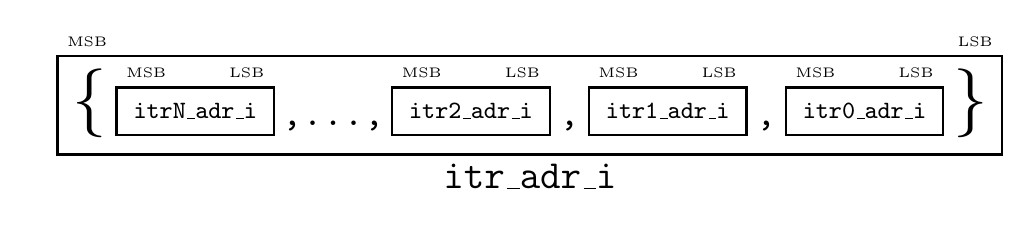
\begin{tikzpicture}
      \node [left] at (1,1.4) {\Huge{\texttt{ \{ }}};
      
      \draw [thick] (1,1) rectangle (3,1.6);
      \node at (2,1.3) {\small{\texttt{itrN\_adr\_i}}};
      \node [above right] at (1,1.6) {\tiny{MSB}};
      \node [above left]  at (3,1.6) {\tiny{LSB}};

      \node [below] at (3.75,1.3) {\Large{\texttt{,...,}}};
     
      \draw [thick] (4.5,1) rectangle (6.5,1.6);
      \node at (5.5,1.3) {\small{\texttt{itr2\_adr\_i}}};
      \node [above right] at (4.5,1.6) {\tiny{MSB}};
      \node [above left]  at (6.5,1.6) {\tiny{LSB}};

      \node [below] at (6.75,1.3) {\Large{\texttt{,}}};

      \draw [thick] (7,1) rectangle (9,1.6);
      \node at (8,1.3) {\small{\texttt{itr1\_adr\_i}}};
      \node [above right] at (7,1.6) {\tiny{MSB}};
      \node [above left]  at (9,1.6) {\tiny{LSB}};

      \node [below] at (9.25,1.3) {\Large{\texttt{,}}};

      \draw [thick] (9.5,1) rectangle (11.5,1.6);
      \node at (10.5,1.3) {\small{\texttt{itr0\_adr\_i}}};
      \node [above right] at (9.5,1.6) {\tiny{MSB}};
      \node [above left]  at (11.5,1.6) {\tiny{LSB}};

      \node [right] at (11.5,1.4) {\Huge{\texttt{\} }}};

      \draw [thick] (0.25,0.75) rectangle (12.25,2);
      \node [above right] at (0.25,2) {\tiny{MSB}};
      \node [above left]  at (12.25,2) {\tiny{LSB}};

      \node [below] at (6.25,0.75) {\Large{\texttt{itr\_adr\_i}}};
    \end{tikzpicture}
    }
    \caption{Concatination of Interface signals}
    \label{sig:concat}
  %\end{center}
\end{figure}

\subsection{Address Region Descriptors}

\begin{description}[style=nextline]
  
\item[\texttt{region\_adr\_i}] Target region descriptors (base addresses). \\
  
  The address range of each bus target is determined by a base address and an address mask.
  An address \texttt{itr\_adr\_i} is within the range of the $n$-th bus target if 
  \begin{center}
    \texttt{itr\_adr\_i[ADR\_WIDTH-1:0] |
      region\_msk\_i[(ADR\_WIDTH*($n$+1))-1:ADR\_WIDTH*$n$]} \\
    $\equiv$ \\
    \texttt{region\_adr\_i[(ADR\_WIDTH*($n$+1))-1:ADR\_WIDTH*$n$] |
      region\_msk\_i[(ADR\_WIDTH*($n$+1))-1:ADR\_WIDTH*$n$]} \\
  \end{center}

\item[\texttt{region\_msk\_i}]  Target region descriptors (address masks). \\
  See \texttt{region\_adr\_i}. 
   
\end{description}

\subsection{General Signals (SYSCON)}

\begin{description}[style=nextline]

\item[\texttt{clk\_i}] Common clock input for all Wishbone interfaces.\\  
  This clock input  corresponds to signal \texttt{CLK\_I} of the Wishbone specification~\cite{wishbone}.

\item[\texttt{itr\_clk\_i}] Clock input for all initiator busses. \\
  Target busses must be clocked by synchronous and subdivided clock.
  This clock input corresponds to signal \texttt{CLK\_I} of the Wishbone specification~\cite{wishbone}.

\item[\texttt{tgt\_clk\_i}] Clock input for all target busses. \\
  Initiator busses must be clocked by synchronous and subdivided clock.
  This clock input corresponds to signal \texttt{CLK\_I} of the Wishbone specification~\cite{wishbone}.

\item[\texttt{itr2tgt\_sync\_i}] Clock phase indicator for for the \nameref{decel} component. \\
    This signal indicates a common positive clock edge of the initiator clock and the synchronous and subdivided
    target clock (see \figref{sig:itr2tgtsync:fig}). 

  \begin{figure}[H]
    \begin{center}
      \begin{tikztimingtable}[timing/slope=0.8]
        \texttt{itr\_clk\_i}      & 15{4c}  \\
        \texttt{tgt\_clk\_i}      & 4c7{8c} \\
        \texttt{itr2tgt\_sync\_i} & 2H7{8t} \\
        \extracode
        \vertlines[thin, dotted]{2,6,...,\twidth}
      \end{tikztimingtable}
      \caption{\texttt{itr2tgt\_sync\_i} Timing Example}
      \label{sig:itr2tgtsync:fig}
    \end{center}
  \end{figure}
  
\item[\texttt{tgt2itr\_sync\_i}] Clock phase indicator for for the \nameref{accel} component. \\
  This signal indicates a common positive clock edge of the target clock and the synchronous and subdivided
  initiator clock (see \figref{sig:tgt2itrsync:fig}).

  \begin{figure}[H]
    \begin{center}
      \begin{tikztimingtable}[timing/slope=0.8]
        \texttt{itr\_clk\_i}      &  5{12c}         \\
        \texttt{tgt\_clk\_i}      & 15{4c}          \\
        \texttt{itr2tgt\_sync\_i} &  4t8t16t8t16t4H \\
        \extracode
        \vertlines[thin, dotted]{2,6,...,\twidth}        
      \end{tikztimingtable}
      \caption{\texttt{tgt2itr\_sync\_i} Timing Example}
      \label{sig:tgt2itrsync:fig}
    \end{center}
  \end{figure}

\item[\texttt{async\_rst\_i}] Optional asynchronous reset input for all sequential logic. \\
  This reset signal may assert asynchronously, but must deassert synchronously. If no
  asynchrounous reset is implemented, this input must be tied to zero.

\item[\texttt{sync\_rst\_i}] Synchronous reset input. \\
  For WbXBC components, this synchronous reset is not required, if an asynchronous reset is provided.
  If no synchrounous reset is implemented, this input must be tied to zero.
  This reset input corresponds to signal \texttt{RST\_I} of the Wishbone specification~\cite{wishbone}.
 
\end{description}

\subsection{Initiator Bus Signals}

\begin{description}[style=nextline]

\item[\texttt{itr\_cyc\_i}] Cycle indicator input. \\
  This input signal corresponds to signal \texttt{CYC\_I} of the Wishbone specification~\cite{wishbone}.

\item[\texttt{itr\_stb\_i}] Strobe input. \\
  This input signal corresponds to signal \texttt{STB\_I} of the Wishbone specification~\cite{wishbone}.

\item[\texttt{itr\_we\_i}] Write enable input. \\
  This input signal corresponds to signal \texttt{WE\_I} of the Wishbone specification~\cite{wishbone}.

\item[\texttt{itr\_lock\_i}] Cycle lock input. \\   
  This input signal corresponds to signal \texttt{LOCK\_I} of the Wishbone specification~\cite{wishbone}.
    
\item[\texttt{itr\_sel\_i}] Write data select inputs. \\
  These input signals correspond to bus \texttt{SEL\_I} of the Wishbone specification~\cite{wishbone}.
    
\item[\texttt{itr\_adr\_i}] Address bus. \\
  These input signals correspond to bus \texttt{ADR\_I} of the Wishbone specification~\cite{wishbone}.

\item[\texttt{itr\_dat\_i}] Write data bus. \\
  These input signals correspond to bus \texttt{DAT\_I} of the Wishbone specification~\cite{wishbone}.

\item[\texttt{itr\_tga\_i}] Address bus tags. \\
  These input signals correspond to bus \texttt{TGA\_I} of the Wishbone specification~\cite{wishbone}.

\item[\texttt{itr\_tgc\_i}] Cycle tags. \\
  These input signals correspond to bus \texttt{TGC\_I} of the Wishbone specification~\cite{wishbone}.

\item[\texttt{itr\_tgd\_i}] Write data tags. \\
  These input signals correspond to bus \texttt{TGD\_I} of the Wishbone specification~\cite{wishbone}.

\item[\texttt{itr\_ack\_o}] Acknowlede output. \\
  This output signal corresponds to signal \texttt{ACK\_O} of the Wishbone specification~\cite{wishbone}.
 
\item[\texttt{itr\_err\_o}] Error indicator output. \\
  This output signal corresponds to signal \texttt{ERR\_O} of the Wishbone specification~\cite{wishbone}.

\item[\texttt{itr\_rty\_o}] Retry output. \\
  This output signal corresponds to signal \texttt{RTY\_O} of the Wishbone specification~\cite{wishbone}.
  For all WbXbc components this signal serves as indicator for a lost bus arbitration.

\item[\texttt{itr\_stall\_o}] Pipeline stall output. \\
  This output signal corresponds to signal \texttt{STALL\_O} of the Wishbone specification~\cite{wishbone}.

\item[\texttt{itr\_dat\_o}] Read data bus. \\
  These output signals correspond to bus \texttt{DAT\_O} of the Wishbone specification~\cite{wishbone}.

\item[\texttt{itr\_tgd\_o}] Read data tags. \\
  These output signals correspond to bus \texttt{TGD\_O} of the Wishbone specification~\cite{wishbone}.

\end{description}

\subsection{Target Bus Signals}

\begin{description}[style=nextline]

\item[\texttt{tgt\_cyc\_o}] Cycle indicator output. \\
  This output signal corresponds to signal \texttt{CYC\_O} of the Wishbone specification~\cite{wishbone}.

\item[\texttt{tgt\_stb\_o}] Strobe output. \\   
  This output signal corresponds to signal \texttt{STB\_O} of the Wishbone specification~\cite{wishbone}.

\item[\texttt{tgt\_we\_o}]  Write enable output. \\
  This output signal corresponds to signal \texttt{WE\_O} of the Wishbone specification~\cite{wishbone}.

\item[\texttt{tgt\_lock\_o}]  Cycle lock output. \\
  This output signal corresponds to signal \texttt{LOCK\_O} of the Wishbone specification~\cite{wishbone}.

\item[\texttt{tgt\_sel\_o}] Write data select outputs. \\    
  These output signals correspond to bus \texttt{SEL\_O} of the Wishbone specification~\cite{wishbone}.

\item[\texttt{tgt\_adr\_o}] Address bus. \\   
  These output signals correspond to bus \texttt{ADR\_O} of the Wishbone specification~\cite{wishbone}.

\item[\texttt{tgt\_dat\_o}] Write data bus. \\    
  These output signals correspond to bus \texttt{DAT\_O} of the Wishbone specification~\cite{wishbone}.

\item[\texttt{tgt\_tga\_o}] Address bus tags. \\   
  These output signals correspond to bus \texttt{TGA\_O} of the Wishbone specification~\cite{wishbone}.

\item[\texttt{tgt\_tgc\_o}] Cycle tags. \\    
  These output signals correspond to bus \texttt{TGC\_O} of the Wishbone specification~\cite{wishbone}.

\item[\texttt{tgt\_tgd\_o}] Write data tags. \\  
  These output signals correspond to bus \texttt{TGD\_O} of the Wishbone specification~\cite{wishbone}.

\item[\texttt{tgt\_ack\_i}] Acknowlede input. \\   
  This input signal corresponds to signal \texttt{ACK\_I} of the Wishbone specification~\cite{wishbone}.

\item[\texttt{tgt\_err\_i}] Error indicator input. \\  
  This input signal corresponds to signal \texttt{ERR\_I} of the Wishbone specification~\cite{wishbone}.

\item[\texttt{tgt\_rty\_i}] Retry input. \\  
  This output signal corresponds to signal \texttt{RTY\_I} of the Wishbone specification~\cite{wishbone}.
  For all WbXbc components this signal serves as indicator for a lost bus arbitration.

\item[\texttt{tgt\_stall\_i}] Pipeline stall input. \\
  This input signal corresponds to signal \texttt{STALL\_I} of the Wishbone specification~\cite{wishbone}.

\item[\texttt{tgt\_dat\_i}] Read data bus. \\ 
  These input signals correspond to bus \texttt{DAT\_I} of the Wishbone specification~\cite{wishbone}.

\item[\texttt{tgt\_tgd\_i}] Read data tags. \\
  These input signals correspond to bus \texttt{TGD\_I} of the Wishbone specification~\cite{wishbone}.

\end{description}

